\documentclass[10pt, a4paper]{scrartcl}
% Packages
%\usepackage{stix}
\usepackage[margin=1.5in]{geometry}
\usepackage{index}
\makeindex
\usepackage[utf8]{inputenc}
\usepackage[T1]{fontenc}
\usepackage{varwidth}
\usepackage{amsmath, amssymb}
\usepackage{esint}
\usepackage{titlesec}
\usepackage{xcolor}
\usepackage{titling}
\usepackage{braket}
\usepackage{tensor}
\usepackage[linktocpage]{hyperref}
\usepackage{pgfplots}
\usepackage{multicol}
\setlength{\columnsep}{2em}
\usepackage{caption}
\usepackage{amsthm}
\usepackage{import}
\usepackage{cancel}
\usepackage{caption}
\usepackage{tcolorbox}
\usepackage{nicematrix}
\usepackage{mathrsfs}
\usepackage{mathtools}
\usepackage{enumerate}
\usepackage{graphicx}
\usepackage{lipsum}
\usepackage[italian]{babel}


%Captions
\captionsetup[figure]{font=footnotesize,labelfont=footnotesize}
\captionsetup[table]{font=footnotesize,labelfont=footnotesize}
%Titlesec
\titleformat{\section}
{\fontsize{15}{20}\sffamily\scshape}
{\normalfont\color{gray}{\fontsize{20}{20}\selectfont\thesection}}
{0.7em}
{}
\hypersetup{colorlinks,breaklinks, linkcolor=[RGB]{74, 122, 164}}

\newcommand\vertarrowbox[3][6ex]{%
  \begin{array}[t]{@{}c@{}} #2 \
  \left\uparrow\vcenter{\hrule height #1}\right.\kern-\nulldelimiterspace\
  \makebox[0pt]{\scriptsize#3}
  \end{array}%
}
\definecolor{asdf}{HTML}{4a7aa4}
% Personalizza la formattazione della subsection
\titleformat{\subsection}[block]{\fontsize{12}{20}\bfseries}{\normalfont\thesubsection}{.5em}{}


% Personalizza la formattazione della subsubsection
\titleformat{\subsubsection}[block]{\fontsize{10}{20}\bfseries}{\normalfont\thesubsubsection}{.5em}{}

% Maketitle customization
\renewcommand{\maketitle}{
\begin{center}
{\sffamily
{\fontsize{20}{20}\selectfont\MakeUppercase\thetitle}}

\vspace{0.2in}

{\large\scshape\sffamily\theauthor}
\end{center}
}

% Titles 
\title{Note di\\ \vspace{.1in} Meccanica Quantistica}
\author{Manuel Deodato}
\date{}



%Evaluate symbol
\DeclareMathOperator{\di}{d\!}
\newcommand*\Eval[3]{\left.#1\right\rvert_{#2}^{#3}}

%%%%%%% Numero delle equazioni in formato a.b
\numberwithin{equation}{subsection}
%%%%%

%%%%%%%%%% Personalizzazione numeri lista
\renewcommand{\theenumi}{(\arabic{enumi})}

%%%%%%%%%% Medie con integrali multipli
\def\Yint#1{\mathchoice
    {\YYint\displaystyle\textstyle{#1}}%
    {\YYint\textstyle\scriptstyle{#1}}%
    {\YYint\scriptstyle\scriptscriptstyle{#1}}%
    {\YYint\scriptscriptstyle\scriptscriptstyle{#1}}%
      \!\iint}
\def\YYint#1#2#3{{\setbox0=\hbox{$#1{#2#3}{\iint}$}
    \vcenter{\hbox{$#2#3$}}\kern-.51\wd0}}
\def\longdash{{-}\mkern-3.5mu{-}} 
   % consider using "\mkern-7.5mu" if esint package is loaded
\def\tiltlongdash{\rotatebox[origin=c]{15}{$\longdash$}}
\def\fiint{\Yint\tiltlongdash}

\def\Zint#1{\mathchoice
    {\YYint\displaystyle\textstyle{#1}}%
    {\YYint\textstyle\scriptstyle{#1}}%
    {\YYint\scriptstyle\scriptscriptstyle{#1}}%
    {\YYint\scriptscriptstyle\scriptscriptstyle{#1}}%
      \!\iiint}
      \def\tilongdash{\mkern6mu{-}\mkern-4mu{-}\mkern-5mu{-}} 
   % consider using "\mkern-7.5mu" if esint package is loaded
\def\titiltlongdash{\rotatebox[origin=c]{15}{$\tilongdash$}}
\def\fiiint{\Zint\titiltlongdash}


%%%% Table of contents

\usepackage[titles]{tocloft}

\renewcommand{\cftdot}{}
\usepackage{titletoc}
%\setcounter{tocdepth}{2}

%%%%%%%%%%%%%%%% Toc style

% Personalizzazione scritta indice


% Font
\usepackage[osf]{newpxtext}

\usepackage{sansiwona}


% Ambienti
\newtheoremstyle{style1}% name of the style to be used
{15pt}% measure of space to leave above the theorem. E.g.: 3pt
{15pt}% measure of space to leave below the theorem. E.g.: 3pt
{\normalfont}% name of font to use in the body of the theorem
{}% measure of space to indent
{\sffamily\scshape\bfseries}% name of head font
{}% punctuation between head and body
{ }% space after theorem head; " " = normal interword space
{\thmname{#1}\thmnumber{ #2}{\thmnote{~--- #3}}.\newline}




\theoremstyle{style1}
\newtheorem{teorema}{Teorema}[section]
\newtheorem{corollario}{Corollario}[teorema]
\newtheorem{lemma}{Lemma}[teorema]
\newtheorem{definizione}{Definizione}[section]
\newtheorem{osservazione}{Osservazione}[section]
\newtheorem{notazione}{Notazione}[section]
\newtheorem{esempio}{Esempio}[section]
\newtheorem{esercizio}{Esercizio}[section]

\renewcommand\qedsymbol{$\blacksquare$}

\newenvironment{svolgimento}{\renewcommand\qedsymbol{$\spadesuit$}\begin{proof}[Svolgimento]}{\end{proof}}

%% Generic box
\newtcolorbox{eqbox}[1][]
{
colback=gray!10,
arc=0pt,
boxrule=0pt,
title=#1
}

 \newenvironment{boxenv}[1][]{
    \begin{eqbox}[#1]
    }{
   \end{eqbox}
}








%%%%%%%%%%%%%%%%%%%%%%%%%%%%%%%%%%%%%%%%%%%%%%%%%%%%%%%%%%%%%%%%%%%%%%%%

\begin{document}
\maketitle
\vspace{25em}
\begin{figure}[h!]
	\centering
	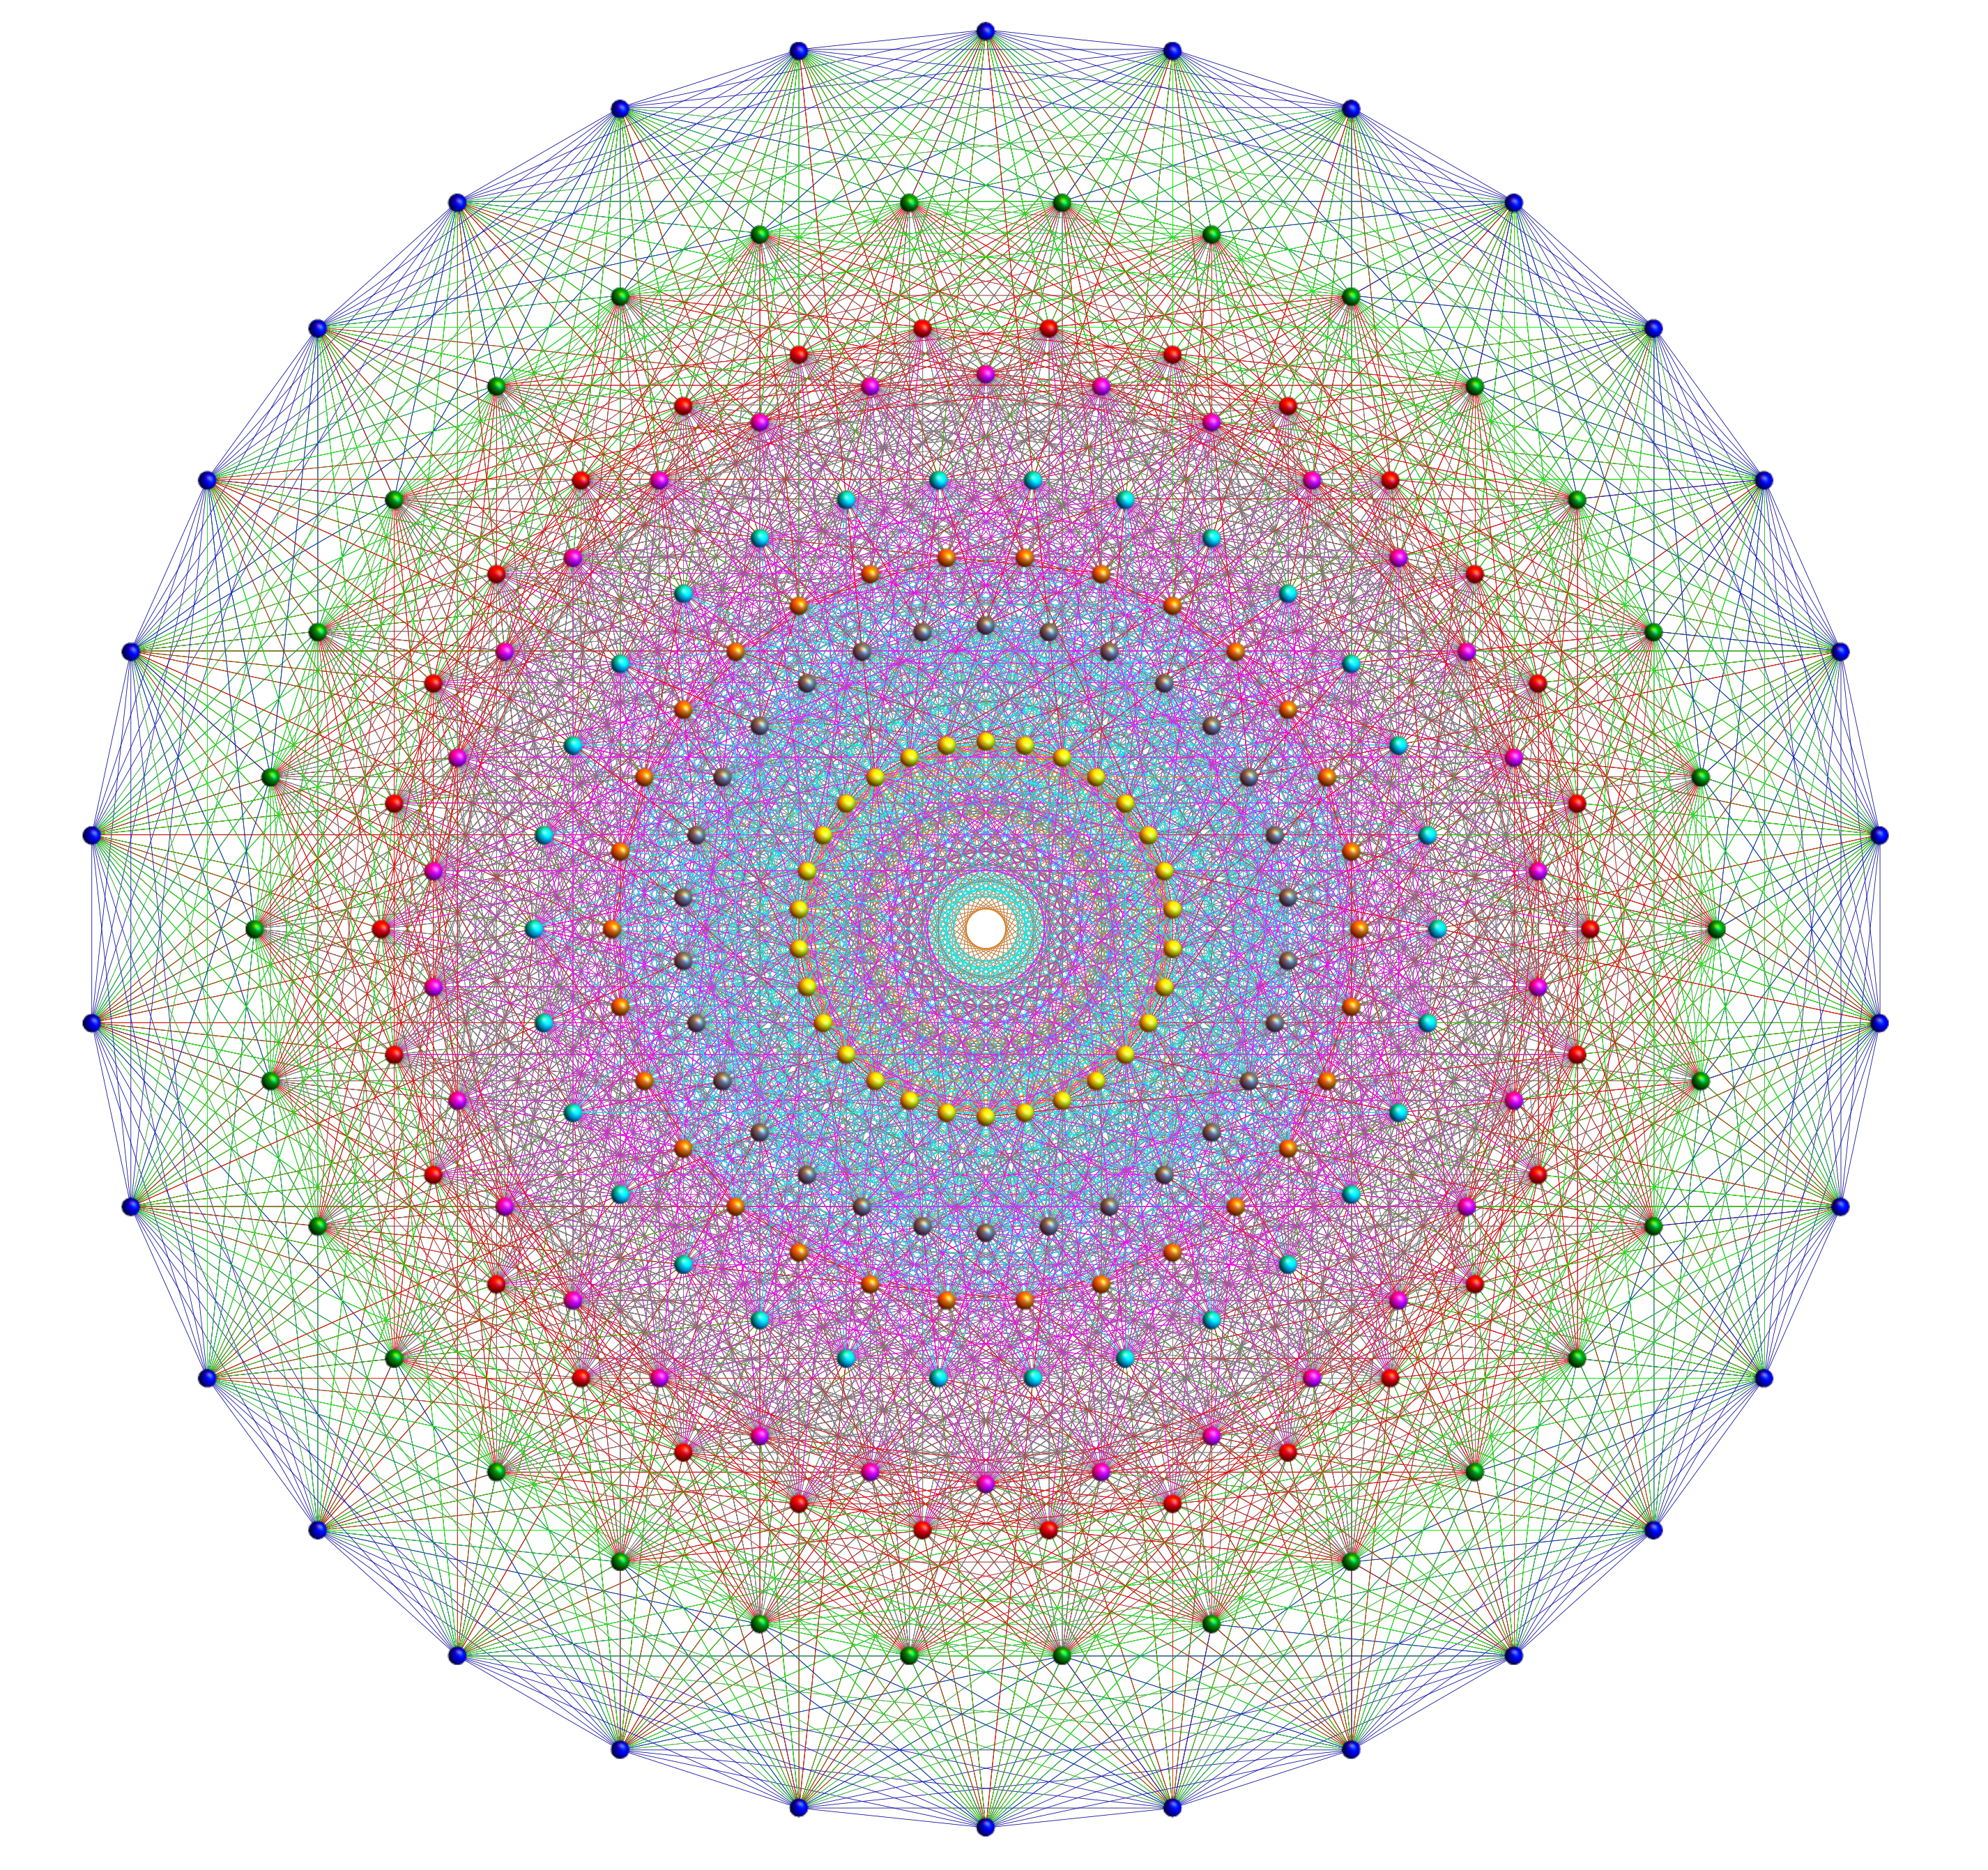
\includegraphics[width=1\columnwidth]{front.jpg}
\end{figure}
\newpage
\tableofcontents 
\newpage
\section{Struttura matematica della meccanica quantistica}
\subsection{Introduzione}
\begin{definizione}
	[Prodotto scalare]
	Per $V$ spazio vettoriale su $\mathbb{C}$ e $\psi ,\phi \in V$, si definisce $\left\langle \cdot ,\cdot  \right\rangle : V\times V \to \mathbb{C}$ come:
	\begin{itemize}
		\item $\left\langle \psi ,\phi  \right\rangle\in \mathbb{C}$;
		\item $\left\langle \psi ,\phi  \right\rangle= \left\langle \phi ,\psi  \right\rangle^*$;
		\item $\left\langle \psi, c_1\phi_1 + c_2\phi_2 \right\rangle = c_1\left\langle \psi ,\phi_1 \right\rangle + c_2 \left\langle \psi , \phi_2 \right\rangle$, con $c_1,c_2 \in \mathbb{C}$;
		\item $\left\langle \phi ,\phi  \right\rangle\ge 0$ e $\left\langle \phi ,\phi  \right\rangle=0 \iff \phi =0$.
	\end{itemize}
\end{definizione}
\noindent Dato $\phi \in V$, questo induce la \textbf{norma}:
\begin{equation}
	\left\lVert \phi  \right\rVert \overset{\text{def}}{=} \sqrt{\left\langle \phi ,\phi  \right\rangle} 
\end{equation}
Si ricordano le seguenti disuguaglianze:
\begin{equation}
	\begin{split}
		&\text{\textbf{Schwarz}: } \left\lvert \left\langle \phi ,\psi  \right\rangle \right\rvert ^2 \le  \left\langle \phi ,\phi  \right\rangle\left\langle \psi ,\psi  \right\rangle\\
		&\text{\textbf{Triangolare}: } \left\lVert \phi + \psi  \right\rVert \le  \left\lVert \psi  \right\rVert +\left\lVert \phi  \right\rVert 
	\end{split}
\end{equation}
\begin{teorema}
	[Teorema di Riesz]
	Dato $T$ operatore lineare limitato agente su spazio di Hilbert $\mathcal{H}$, allora $\exists f \in \mathcal{H}:\forall \phi \in \mathcal{H}\Rightarrow T(\phi )\equiv \left\langle f,\phi  \right\rangle$. Inoltre, $\left\lVert T \right\rVert = \left\lVert f \right\rVert $.
\end{teorema}
\begin{osservazione}
	[Funzionali e operatori]
	Un funzionale lineare \`e un operatore lineare $F$ che agisce su uno spazio vettoriale $V$ su $\mathbb{K}$ e restituisce un valore nel campo; formalmente: $F:V\to \mathbb{K}$. In generale, gli operatori non restituiscono valori in $\mathbb{K}$, mentre i funzionali s\`i.	

Gli operatori rappresentano gli osservabili, mentre i funzionali sono usati per calcolare aspettazione e probabilit\`a.
\end{osservazione}
\subsubsection{Notazione bra-ket}
Sia $V$ uno spazio vettoriale e $V'$ il suo duale; si definiscono:
\begin{itemize}
	\item per $\phi \in V \longrightarrow \ket{\phi } \in V$;
	\item per $F \in  V' \longrightarrow \bra{F} \in V'$.
\end{itemize}
Per Riesz, per qualche $f \in V$:
\begin{equation}
	\braket{F|\phi } \overset{\text{def}}{=}F(\phi ) = \left\langle f,\phi  \right\rangle \Rightarrow F(\phi ) \leftrightarrow \braket{f|\phi}
\end{equation}
Visto che $\braket{\phi |\psi } = \left\langle \phi ,\psi  \right\rangle$, allora: 
\begin{equation}
	\bra{c\phi } = c^* \bra{\phi } \longleftrightarrow \ket{c\phi } = c \ket{\phi } 
\end{equation}
\subsubsection{Operatori}
Si considerano vettori, o \textbf{stati}, in uno spazio di Hilbert $\mathcal{H}$. Un operatore che agisce su tale spazio \`e definito come $\hat{A}: \mathcal{H}\to \mathcal{H}$, quindi $\hat{A}\ket{\phi } \in \mathcal{H}$. Gli operatori di interesse saranno \textbf{lineari}.

Se $\hat{A}$ \`e limitato (quindi continuo), dato $\ket{\psi } \in \mathcal{H}$, con $\left\{ \phi _i \right\} $ base ortonormale:
\begin{equation*}
	\begin{cases}
		 \hat{A}\ket{\psi } = \ket{\phi } = \sum_{i=1}^{+\infty} c_i \ket{\phi _i}  \\
		\\
		 \hat{A}\ket{\psi } = \sum_{i=1}^{+\infty} b_i \hat{A}\ket{\phi _i} 
	\end{cases}
\end{equation*}
si nota che
\begin{equation}
	\braket{\phi _j|\hat{A}\psi } =\bra{\phi _j} \left(\sum_{i=1}^{+\infty} b_i \hat{A} \ket{\phi _i} \right)  = \sum_{i=1}^{+\infty} b_i\underbracket{\braket{\phi _j|\hat{A}|\phi _i}}_{\equiv A_{ji} } 
\end{equation}
dove $A_{ji} $ \`e un elemento di matrice; infatti
\begin{equation*}
		 \braket{\phi _j|\phi } = \braket{\phi _j|\hat{A}|\psi } = \sum_{i=1}^{+\infty}c_i \braket{\phi _j|\phi _i} = c_j
\end{equation*}
da cui, unendo le uguaglianze:
\begin{equation*}
\sum_{i=1}^{+\infty} A_{ji} b_i = c_j	
\end{equation*}
Sia $\hat{A}$ lineare; l'aggiunto \`e $\hat{A}^\dagger $ e tale che $\langle \phi , \hat{A}\psi  \rangle= \langle \hat{A}^\dagger \phi ,\psi  \rangle$. Allora, in notazione bra-ket:
\begin{equation}
	\bra{w} = \bra{\phi } \hat{A}^\dagger \longleftrightarrow \ket{w} = \hat{A}\ket{\phi } 
\end{equation}
Inoltre 
\begin{boxenv}[]
\begin{equation}
	\begin{split}
		&\left\langle \psi ,\phi  \right\rangle^* = \left\langle \phi ,\psi  \right\rangle \implies \braket{\psi |\phi } ^* = \braket{\phi |\psi }\\
		& \Rightarrow \braket{\psi  |\hat{A}^\dagger |\phi } ^* = \braket{\phi |\hat{A}|\psi } 
	\end{split}
\end{equation}
\end{boxenv}
\noindent Infine, se $\left\{ \phi _i \right\} $ base ortonormale:
\begin{boxenv}[]
\begin{equation}
	A^\dagger _{ij} = \braket{\phi _i|\hat{A}^\dagger |\phi _j} = \braket{\phi _j|\hat{A}|\phi _i} ^* = A_{ji} ^* \Rightarrow A^\dagger = (A^\top)^*
\end{equation}
\end{boxenv}
\noindent Da questo, segue:
\begin{equation}
	(AB)^\dagger = B^\dagger A^\dagger; \ (cA)^\dagger = c^* A^\dagger 
\end{equation}
\subsubsection{Operatori autoaggiunti}
\begin{definizione}
	[Operatore autoaggiunto]
	Sia \( \mathcal{H} \) uno spazio di Hilbert complesso e sia \( A \) un operatore lineare definito su un dominio \( \operatorname{Dom} (A) \subseteq \mathcal{H} \). L'operatore \( A \) si dice \textbf{autoaggiunto} se soddisfa le seguenti condizioni:

\begin{enumerate}
    \item \textbf{Densità del dominio:} il dominio \( \text{Dom}(A) \) è denso nello spazio di Hilbert \( \mathcal{H} \), ovvero:
    \[
    \overline{\text{Dom}(A)} = \mathcal{H}.
    \]

    \item \textbf{Simmetria:} per ogni \( \psi, \phi \in \text{Dom}(A) \),
    \[
    \langle \psi, A \phi \rangle = \langle A \psi, \phi \rangle.
    \]

    \item \textbf{Uguaglianza con l'aggiunto:} il dominio di \( A \) coincide con quello del suo aggiunto \( A^\dagger \), e i due operatori coincidono, ovvero:
    \[
    \text{Dom}(A) = \text{Dom}(A^\dagger) \quad \text{e} \quad A = A^\dagger.
    \]
\end{enumerate}
\end{definizione}
\noindent Essendo $\hat{A}= \hat{A}^\dagger $, si ha $A_{ij} = (A_{ij} ^*)^\top$. Questi sono sempre diagonalizzabili, quindi hanno base ortonormale di autovettori. Visto che $\braket{\phi _1|\hat{A}|\phi _2} = \braket{\phi _2|\hat{A}|\phi _1} ^*$, allora $\braket{\psi |\hat{A}|\psi } \in \mathbb{R}$ ed \`e il \textbf{valore di aspettazione}.

Sia $\ket{\psi } $ autostato di $\hat{A}$ autoaggiunto; allora $\hat{A} \ket{\psi } = a \ket{\psi } \Rightarrow \bra{\psi } \hat{A}=  \bra{\psi } a^*$. Si nota, per\`o, che:
\begin{equation}
	a \braket{\psi |\psi } = \braket{\psi |\hat{A}|\psi } = \braket{\psi |\hat{A}^\dagger |\psi } = a^* \braket{\psi |\psi } \iff a=a^* \Rightarrow a \in \mathbb{R}
\end{equation}
Siano $\ket{\psi_1} , \ket{\psi_2} $ tali che $\hat{A}\ket{\psi_1} = a_1 \ket{\psi_1} $ e $\hat{A}\ket{\psi_2} = a_2\ket{\psi_2} $, con $a_1\neq a_2$; allora:
\begin{equation}
	\begin{split}
		& a_2 \braket{\psi_1|\psi_2} = \braket{\psi_1|\hat{A}|\psi_2} = \braket{\psi_1|\hat{A}^\dagger |\psi_2} = a_1^* \braket{\psi_1|\psi_2}= a_1 \braket{\psi_1|\psi_2} \\
		&\Rightarrow (a_2-a_1) \braket{\psi_1|\psi_2}=0 \iff \ket{\psi_1} \perp \ket{\psi_2} 
	\end{split}
\end{equation}
\subsubsection{Commutatori}
\begin{definizione}
	[Commutatore]
	Siano $\hat{A},\hat{B}$ due operatori; il commutatore \`e: $[ \hat{A},\hat{B} ] \overset{\text{def}}{=} \hat{A}\hat{B} - \hat{B}\hat{A}$. Quindi se $\hat{A},\hat{B}$ commutano, si ha $[ \hat{A},\hat{B} ] =0$.
\end{definizione}
\begin{teorema}
	[Spettro comune]
	Se $\hat{A},\hat{B}$ sono autoaggiunti e commutano, allora condividono una base di autovettori.
\end{teorema}
\subsection{Prodotto esterno}
Applicazione $\rho : V \times  V \to \mathcal{O}$, con $\mathcal{O}$ spazio degli operatori lineari. Un esempio di prodotto esterno \`e l'operatore lineare
\begin{boxenv}[]
\begin{equation}
	\hat{O} = \ket{\psi } \bra{\phi } : V \to V
\end{equation}
\end{boxenv}
\noindent Si nota che:
\[
\begin{split}
	&\braket{v|\hat{O}w} = \braket{v|(\ket{\psi } \bra{\phi } ) w} = \braket{v|\psi } \braket{\phi |w}=\braket{ \hat{O}^\dagger v|w} \iff O^\dagger = \ket{\phi}\bra{\psi  }  
\end{split}
\] 
\subsubsection{Proiettori}

Operatore $\hat{P}$ tale che $\hat{P}^2 = \hat{P}$. Un esempio \`e $\hat{P}=\ket{\psi } \bra{\psi } $, con $\left\lVert \psi  \right\rVert =1$ perch\'e:
\[
\hat{P}^2 = \ket{\psi } \braket{\psi |\psi } \bra{\psi } =\ket{\psi } \bra{\psi } \equiv \hat{P}
\] 
\subsubsection{Completezza di una base e valore di aspettazione di un osservabile}

Un insieme ortonormale $\left\{ \ket{\phi_i }  \right\} $ si dice completo se:
\begin{boxenv}[]
\begin{equation}
	\sum_{i=1}^{+\infty} \ket{\phi _i} \bra{\phi _i} = \operatorname{Id} 
\end{equation}
\end{boxenv}
\noindent Un insieme ortonormale completo \`e una base ortonormale di $\mathcal{H}$, quindi permette di scomporre ogni stato in una combinazione lineare.
\subsubsection{Cambiamento di base}
Siano $\left\{ \ket{\phi _i}  \right\}_i , \ \left\{ \ket{\psi _i}  \right\}_i $ basi ortonormali. Si esprime una in funzione dell'altra:
\begin{equation}
	\ket{\psi _i} = \left(\sum_{j=1}^{+\infty} \ket{\phi _j} \bra{\phi _j} \right) \ket{\psi _i} = \sum_{j=1}^{+\infty} \braket{\phi _j|\psi _i} \ket{\phi _j} \equiv \sum_{j=1}^{+\infty} S^* _{ij} \ket{\phi _j} 
\end{equation}
Per $\varphi $ generico stato: $\ket{\varphi } = \sum_{i=1}^{+\infty} a_i \ket{\phi _i} = \sum_{i=1}^{+\infty} b_i \ket{\psi _i} $; allora:
\begin{equation}
	\begin{cases}
		\displaystyle b_i=\braket{\psi _i|\varphi } = \sum_{j=1}^{+\infty} a_j \braket{\psi _i|\phi _j} \equiv \sum_{j=1}^{+\infty} S_{ij} a_j\\
		\\
		\displaystyle a_i = \braket{\phi _i|\varphi } =\sum_{j=1}^{+\infty} b_j \braket{\phi _i|\psi _j} \equiv \sum_{j=1}^{+\infty} S_{ji}^* b_j
	\end{cases}
\end{equation}
Ora, essendo le due basi ortonormali:
\begin{equation}
	\delta _{ij} = \Braket{\phi _i|\left(\sum_{k=1}^{+\infty} \left\lvert \psi _k \right\rangle\left\langle \psi _k \right\rvert \right) \phi _j} = \sum_{k=1}^{+\infty} \braket{\phi _i|\psi _k} \braket{\psi _k|\phi _j} = \sum_{k=1}^{+\infty} S_{ki} ^* S_{kj} 
\end{equation}
da cui $S^\dagger S = \operatorname{Id} $.

\subsection{Applicazioni per la meccanica quantistica}

\subsubsection{Rappresentazione delle coordinate}
Uno stato si decompone in maniera diversa a seconda della base; ogni decomposizione \`e una sua diversa \textbf{rappresentazione}. 

Sia $\hat{Q}:\mathcal{H}\to \mathcal{H}$ operatore autoaggiunto \textbf{posizione}\footnote{Indicato anche con $\hat{X}$.}, con $\hat{Q}\ket{x} =x \ket{x} $\footnote{Gli autostati sono le $x$, mentre $\ket{x} $ rappresenta gli autovettori.}. Il suo spettro \`e continuo, quindi la decomposizione spettrale avviene tramite integrale: dato uno stato $\ket{\psi }\in \mathcal{H}$
\begin{equation}
	\ket{\psi } = \int_{-\infty} ^{+\infty} \braket{x|\psi } \ket{x } \ dx \equiv \int_{-\infty} ^{+\infty} \psi (x) \ket{x} \ dx 
\end{equation}
con $\psi (x)$ \textbf{funzione d'onda} dello stato $\ket{\psi } $ e ne indica i coefficienti nella rappresentazione delle coordinate.
\subsubsection{Rappresentazione degli impulsi}
Sia $\hat{p}\ket{p} = p \ket{p} $ operatore impulso (autoaggiunto); per $\ket{\psi } \in \mathcal{H}$:
\begin{equation}
	\ket{\psi } = \int_{-\infty} ^{+\infty} dp \ c(p) \ket{p} \equiv \int_{-\infty} ^{+\infty} dp \ \widetilde{\psi }(p) \ket{p} 
\end{equation}
dove $\widetilde{\psi }(p) $ \`e la funzione d'onda nel dominio degli impulsi e si ottiene trasformando con Fourier $\psi (x)$.
\subsubsection{Misura di un osservabile}
Sia $\hat{A}$ operatore lineare autoaggiunto\footnote{In generale, ogni operatore in meccanica quantistica, almeno quelli associati ad osservabili, sono operatori lineari autoaggiunti.} con autovalori $a_i$ e autovettori $\ket{\lambda _i} $. Assumendo che $\braket{\lambda _i|\lambda _j} = \delta _{ij} $ formino una base ortonormale\footnote{Possono essere sempre costruiti in modo che siano ortonormali.} e dato un generico $\ket{\psi } = \sum_{i=1}^{+\infty}b_i \ket{\lambda _i} $, si nota che :
\begin{equation}
	\braket{\psi |\hat{A}|\psi } = \left[ \sum_{i=1}^{+\infty} b^*_j \bra{\lambda _i}  \right] \left[ \sum_{j=1}^{+\infty} b_j \hat{A}\ket{\lambda _j}  \right]= \sum_{i=1}^{+\infty} \left\lvert b_i \right\rvert ^2 a_i
\end{equation}
\noindent dove si pu\`o vedere $\left\lvert b_i \right\rvert ^2$ come probabilit\`a di ottenere misura $a_i$ da osservabile $\hat{A}$. In questo senso, deve valere:
\[
\sum_{i=1}^{+\infty} \left\lvert b_i \right\rvert ^2 \stackrel{!}{=}1
\] 
Questa condizione \`e verificata dalla normalizzazione di ciascuno stato:
\begin{equation}
		\braket{\psi |\psi } = \left[ \sum_{i=1}^{+\infty} b_i^* \bra{\lambda _i}  \right] \left[ \sum_{j=1}^{+\infty} b_j \ket{\lambda _j}  \right] = \sum_{i,j=1}^{+\infty} b_i^* b_j \braket{\lambda _i|\lambda _j} =\sum_{i=1}^{+\infty} \left\lvert b_i \right\rvert ^2 \stackrel{!}{=}1
\end{equation}
\noindent Per un operatore a spettro continuo $\hat{F}$, con autovettori $\ket{z} $ relativi ad autovalori $z$ e $\ket{\psi } \in \mathcal{H}, \  \ket{\psi } = \int_{-\infty} ^{+\infty} f(z) \ket{z} \ dz, \ f(z) = \braket{z|\psi }$:
\begin{equation}
	\begin{split}
		&\begin{split}
			\braket{\psi| \hat{F}|\psi }&=\int_{-\infty} ^{+\infty} f^*(y) \bra{y}\ dy \int_{-\infty} ^{+\infty} f(z) \hat{F}\ket{z} \ dz\\
						    &= \int_{-\infty} ^{+\infty} \int_{-\infty} ^{+\infty} dydz \ f^*(y) f(z) z\braket{y|z} = \int_{-\infty} ^{+\infty} z\left\lvert f(z) \right\rvert ^2 \ dz
		\end{split}\\
		&\braket{\psi |\psi } = \int_{-\infty} ^{+\infty} \left\lvert f(z) \right\rvert ^2 \ dz \stackrel{!}{=}1 \text{ \textbf{(normalizzazione)} }
	\end{split}
\end{equation}
\subsubsection{Principi della meccanica quantistica}
\begin{enumerate}[(a).]
	\item Uno stato fisico $\ket{\psi } $ \`e un vettore in uno spazio di Hilbert $\mathcal{H}$, $\ell ^2$ o $L^2$. Lo stesso stato pu\`o essere equivalentemente moltiplicato per una fase: $e^{i\alpha } \ket{\psi } $.
	\item Per ogni sistema, ogni stato deve essere tale che $\braket{\psi |\psi } =1$.
	\item Gli osservabili sono operatori lineari autoaggiunti che agiscono su $\mathcal{H}$.
	\item Il valore di aspettazione di un osservabile $\hat{A}$ relativo ad uno stato $\ket{\psi } $ \`e $\braket{\psi |\hat{A}|\psi } $. Se $a_i$ sono autovalori, con $\ket{a_i} $ relativi autovettori, di $\hat{A}$, la probabilit\`a di ottenere la misura $a_i$ (data dal fatto che il sistema \`e nello stato $\ket{a_i} $) \`e $\left\lvert a_i \right\rvert ^2$. 

		Nel caso di operatori con spettri continui, si costruisce la densit\`a di probabilit\`a $P(x) dx = \left\lvert \psi (x) \right\rvert ^2 dx$ (come esempio per operatore posizione $\hat{Q}$) ed \`e probabilit\`a di trovare la particella nell'intervallo spaziale $dx$.
\end{enumerate}
\subsubsection{Spazio di Hilbert proiettivo, sistemi puri e misti}
Ogni stato $\ket{\psi } $ \`e definito a meno di una fase; per eliminare fase globale, si usa lo spazio proiettivo $\mathcal{P}(\mathcal{H}) = \mathcal{H} /\mathord{\sim}$, con $\ket{\psi } \sim e^{i\alpha }  \ket{\psi } $.

Con gli elementi di $\mathcal{P}(\mathcal{H})$ si pu\`o introdurre un \textbf{isomorfismo naturale}\footnote{Isomorfismo che non dipende dalla scelta del rappresentante della classe di equivalenza.} con lo spazio generato dagli operatori $\rho = \ket{\psi } \bra{\psi } $, nel caso di sistemi \textbf{puri}. 

Un sistema quantistico puro, \`e univocamente descritto da un singolo stato $\ket{\psi } $ (quello in cui si trova in un certo istante temporale), quindi il proiettore $\rho  = \ket{\psi } \bra{\psi } $ contiene tutte le informazioni necessarie per una sua descrizione. Un sistema \textbf{misto}, invece, non pu\`o essere descritto tramite un singolo stato perch\'e appartiene a pi\`u stati puri contemporaneamente in una certa proporzione; in questo caso, il proiettore diventa una \textbf{matrice di densit\`a}  con 
\begin{equation}
	\rho = \sum_{i} p_i \ket{\psi _i} \bra{\psi _i} 
\end{equation}
\subsubsection{Proiettore per sistemi puri}
La condizione di normalizzazione \`e:
\begin{equation}
	\operatorname{Tr} \rho = 1
\end{equation}
\begin{boxenv}[]
\begin{proof}
	Se $\ket{\psi } = \sum_{n=1}^{+\infty} c_n \ket{\phi _n} $:
	\begin{equation}
		\begin{split}
			\operatorname{Tr} \rho  &\overset{\text{def}}{=} \sum_{m=1}^{+\infty} \sum_{n=1}^{+\infty} \braket{\phi _m|\rho |\phi _n} \delta _{mn} = \sum_{n=1}^{+\infty} \braket{\phi _n|\rho |\phi _n}  = \sum_{n=1}^{+\infty} \braket{\phi _n|\psi } \braket{\psi |\phi _n} \\
			&=\sum_{n=1}^{+\infty} \left\lvert \braket{\phi _n|\psi }  \right\rvert ^2 = \braket{\psi |\psi }  		\end{split}
	\end{equation}
	dove l'ultima uguaglianza deriva dalla completezza di $\left\{ \ket{\phi _n}  \right\}_n $.
\end{proof}
\end{boxenv}
\noindent Un generico elemento di matrice di $\rho = \ket{\psi } \bra{\psi } $ \`e $\rho _{ij} = c_i c_j^*$, dove $\ket{\psi } = \sum_{i}^{} c_i \ket{\phi _i} $.
\begin{boxenv}
\begin{proof}
	Per conto diretto:
	\begin{equation}
		\begin{split}
			\rho _{ij} &= \braket{\phi _i|\rho |\phi _j} = \braket{\phi _i|\psi } \braket{\psi |\phi _j} = \sum_{m=1}^{+\infty} c_m \braket{\phi _i|\phi _m} \sum_{n=1}^{+\infty} c_n^* \braket{\phi _n|\phi _j} \\
			&=\sum_{m,n=1}^{+\infty} c_m c_n^* \delta _{im} \delta _{jn} = c_ic_j^*
		\end{split}
	\end{equation}
\end{proof}
\end{boxenv}
\noindent Dato $\hat{A}$ osservabile con base di autostati $\left\{ \ket{a_i}  \right\} _i$:
\begin{equation}
	\braket{\psi |\hat{A}|\psi } = \operatorname{Tr} \rho \hat{A}
\end{equation}
\begin{boxenv}[]
\begin{proof}
	Si prende $\psi = \sum_{i}^{} c_i \ket{a _i} $ e $\rho = \ket{\psi } \bra{\psi }  $; allora: 
	\begin{equation}
			\operatorname{Tr} (\rho \hat{A}) \overset{\text{def}}{=} \sum_{i}^{} \braket{a _i|\rho \hat{A}|a _i} = \sum_{i}^{} a_i \braket{a_i|\rho |a_i} = \sum_{i}^{} \lvert c_i \rvert ^2 a_i \equiv \braket{\psi |\hat{A}|\psi } 
	\end{equation}
\end{proof}
\end{boxenv}
\subsubsection{Flusso di probabilit\`a ed equazione di continuit\`a}

Sistema composto da particella in 3D sotto potenziale $V(x)$. Sia $\psi (\mathbf{x} ,t)$ funzione d'onda per stato $\ket{\psi(t) } $. La probabilit\`a di trovare particella in una regione $\Gamma$ dello spazio \`e\footnote{I termini con il potenziale si cancellano perch\'e simmetrici, mentre quelli con $\nabla ^2$ no perch\'e in uno sar\`a derivato $\psi $, nell'altro $\psi ^*$.}:
\begin{equation}
	P_\Gamma (t) \equiv\int_{\Gamma} d^3 x \ \lvert \psi (\mathbf{x} ,t) \rvert ^2 
\end{equation}
Per quanto detto in \S\ref{pice}: $i\hbar  \partial _t \psi (\mathbf{x} ,t) = \left(- \frac{\hbar ^2}{2m} \nabla ^2 + V(\mathbf{x} )\right) \psi (\mathbf{x} ,t)$; evoluzione temporale di $P_\Gamma(t)$ \`e:
\[
\begin{split}
	\partial _t P_\Gamma(t) &= \partial _t \int_{\Gamma}d^3 x \ \psi (\mathbf{x} ,t) \psi ^*(\mathbf{x} ,t) = \int_{\Gamma} \big[\psi ^*(\mathbf{x} ,t) \partial _t \psi (\mathbf{x} ,t) + \psi (\mathbf{x} ,t) \partial _t \psi ^*(\mathbf{x} ,t)\big] \ d^3x \\
				& = \int_{\Gamma} \left[ \psi ^*(\mathbf{x} ,t) \frac{1}{i\hbar } \left(- \frac{\hbar ^2}{2m} \nabla ^2 + V(x) \right) \psi (\mathbf{x} ,t) - \frac{1}{i\hbar } \left(- \frac{\hbar ^2}{2m} \nabla ^2 + V(x) \right) \psi^* (\mathbf{x} ,t)  \right]  \ d^3x \\
				&= \frac{i\hbar }{2m}\int_{\Gamma} \big[\psi ^*(\mathbf{x} ,t) \nabla ^2 \psi (\mathbf{x} ,t) - \psi (\mathbf{x},t) \nabla ^2 \psi ^*(\mathbf{x} ,t) \big]	\ d^3x= \frac{i\hbar }{2m} \int_{\Gamma} \nabla \cdot \big(\psi ^* \nabla \psi - \psi \nabla \psi ^*\big)	\ d^3x
\end{split}
\] 
Definendo \textbf{flusso di probabilit\`a}:
\begin{boxenv}[]
\begin{equation}
	\mathbf{J} = - \frac{i\hbar }{2m} \big( \psi ^* \nabla \psi  - \psi \nabla \psi ^*\big)
\end{equation}
\end{boxenv}
\noindent si ha:
\begin{equation}
	\partial _t P_\Gamma(t) = - \int_{\Gamma} \nabla \cdot \mathbf{J} \ d^3 x 
\end{equation}
da cui si ottiene equazione di continuit\`a:
\begin{boxenv}[]
\begin{equation}
	\partial _t \lvert \psi  \rvert ^2 + \nabla \cdot \mathbf{J} =0
\end{equation}
\end{boxenv}

\newpage	
\section{Introduzione alla meccanica quantistica}
\subsection{Evoluzione temporale}
\subsubsection{Equazione di Shr\"odinger per gli stati}

Variazione temporale dello stato di un sistema: $\ket{\psi (t)} $ o $\ket{\psi ,t} $. Per la funzione d'onda: $\psi (x,t) = \braket{x|\psi (t)} $. Per trovare evoluzione temporale di uno stato, si richiede che:
\begin{enumerate}[(a).]
	\item l'evoluzione sia univocamente determinata da uno stato iniziale $\Rightarrow $ si richiede che nell'equazione compaia al massimo il primo ordine di derivazione $\partial _t\ket{\psi (t)}$;
	\item sperimentalmente, si verifica il principio di sovrapposizione, quindi l'equazione differenziale deve essere lineare.
\end{enumerate}
L'equazione risultante \`e:
\begin{equation}
	i \hbar \partial _t \ket{\psi (t)} = \hat{H}\ket{\psi (t)} 
\end{equation}
$\hat{H}$ \`e un generico operatore che definisce l'evoluzione temporale del sistema. Deve risultare autoaggiunto.
\begin{boxenv}[]
\begin{proof}
	Da $\braket{\psi (t)|\psi (t)} \stackrel{!}{=}1, \ \forall t$:
	\begin{equation}
		\begin{split}
			&0\stackrel{!}{=} \partial _t \braket{\psi (t)|\psi (t)} = \big(\partial _t \bra{\psi (t)} \big)\ket{\psi (t)}  + \bra{\psi (t)} \big(\partial _t\ket{\psi (t)} \big)\\
			&\Rightarrow \frac{i}{\hbar} \braket{\psi (t)|\hat{H}^\dagger |\psi (t)} = \frac{i}{\hbar} \braket{\psi (t)|\hat{H}|\psi (t)} \Rightarrow \hat{H}^\dagger = \hat{H}
		\end{split}
	\end{equation}
\end{proof}
\end{boxenv}
\noindent Questo candida $\hat{H}$ come osservabile
\subsubsection{Soluzione dell'equazione}

La soluzione \`e:
\begin{equation}
	\ket{\psi (t)} = e^{-\frac{i}{\hbar } \hat{H}(t-t_0) } \ket{\psi (t_0)} 
\end{equation}
dove 
\begin{equation*}
	e^{\hat{A}} \overset{\text{def}}{=} 1+ \hat{A}+\frac{1}{2}\hat{A}^2 + \ldots
\end{equation*}
Visto che $\hat{H}$ \`e autoaggiunto, l'esponenziale \`e unitario:
\begin{equation}
e^{- \frac{i}{\hbar} \hat{H}(t-t_0)} e^{\frac{i}{\hbar } \hat{H}(t-t_0)}  = \operatorname{Id} 
\end{equation}
Definendo l'\textbf{evolutore} come l'operatore $\hat{U}(t,t_0)$ tale che $\ket{\psi (t)}  = \hat{U}(t,t_0) \ket{\psi(t_0) } $, risulta $\hat{U}(t,t_0) \hat{U}^\dagger(t,t_0) = \operatorname{Id} $. Se $\hat{H}$ \textbf{indipendente dal tempo}, allora $\hat{U}(t,t_0) = e^{- \frac{i}{\hbar}\hat{H}(t-t_0)} $.
\subsubsection{Equazione di Shr\"odinger per la funzione d'onda}
Per $\left\{ \ket{x}  \right\} $ base ortonormale $\Rightarrow \int_{-\infty} ^{+\infty} dx \ \braket{\psi (t)|x} \braket{x|\psi (t)} =\int_{-\infty}^{+\infty}   dx \ \left\lvert \psi (x,t) \right\rvert ^2 \stackrel{!}{=}1$ per normalizzazione. Nell'eq. di Shr\"odinger:
\begin{equation}
	i \hbar \partial _t \ket{\psi (t)}  = \hat{H} \ket{\psi (t)} \Rightarrow  i\hbar \partial _t \braket{x|\psi (t)} = \braket{x|\hat{H}|\psi (t)} \Rightarrow i\hbar \partial _t \psi (x,t) = \hat{H}\psi (x,t)
\end{equation}
Il passaggio $ \braket{x|\hat{H}|\psi (t)} \stackrel{*}{=} \hat{H}\psi (x,t)$ \`e giustificato con l'accorgimento che gli $\hat{H}$ non sono gli stessi: uno agisce su ket, l'altro su scalare; la definizione di $\hat{H}$ agente su $\psi (x,t)$ \`e:
\[
\braket{x|\hat{H}|\psi (t)} \equiv \int_{-\infty}^{+\infty}  dy\ \braket{x|\hat{H}|y} \braket{y|\psi (t)} \overset{\text{def}}{=} \hat{H} \psi (x,t)
\] 
con $\braket{x|\hat{H}|y} $ \`e l'elemento di matrice dell'Hamiltoniano originale nella rappresentazione delle coordinate. 

Per la soluzione dell'equazione:
\[
	\begin{split}
		&\ket{\psi (t)}  = \hat{U}(t,t_0) \ket{\psi (t_0)} \Rightarrow \braket{x|\psi (t)} = \psi (x,t)= \braket{x|\hat{U}(t,t_0)|\psi (t_0)} \\
		&\Rightarrow \psi (x,t) = \int_{-\infty} ^{+\infty} dy \ \braket{x|\hat{U}(t,t_0)|y} \braket{y|\psi (t_0)} = \int_{-\infty} ^{+\infty} dy \ \hat{U}(x,y,t,t_0) \psi (y,t_0)\\
		&\Rightarrow \psi (x,t) = \hat{U}(t,t_0) \psi (x,t_0)
	\end{split}
\] 
dove, come prima, i due $\hat{U}$ non sono gli stessi.

\subsubsection{Equazione di Shr\"odinger per il proiettore}

Partendo da $\hat{\rho }(t)= \ket{\psi (t)} \bra{\psi (t)} $, si trova:
\begin{equation}
	\begin{split}
		\partial _t \hat{\rho }(t) &= \big[\partial _t \ket{\psi (t)} \big] \bra{\psi (t)} + \ket{\psi (t)} \big[\partial _t \bra{\psi (t)} \big] \\
					   &= - \frac{i}{\hbar } \hat{H} \ket{\psi (t)} \bra{\psi (t)}  + \frac{i}{\hbar } \ket{\psi (t)} \bra{\psi (t)} \hat{H}^\dagger  =-\frac{i}{\hbar }\hat{H} \hat{\rho }(t) + \frac{i}{\hbar }\hat{\rho} (t)\hat{H}\\
					   &= - \frac{i}{\hbar }\left[ \hat{H},\hat{\rho }(t) \right] 
	\end{split}
\end{equation}
\subsection{Evoluzione temporale per gli operatori}
Ci sono tre quadri per vedere il problema:
\begin{enumerate}[(a).]
	\item \textbf{quadro di Shr\"odinger:} solo gli stati dipendono dal tempo, mentre gli operatori no;
	\item \textbf{quadro di Heisenberg:} solo gli operatori dipendono dal tempo;
	\item \textbf{quadro misto (o di interazione):} l'hamiltoniano si divide in $\hat{H} = \hat{H}_0 + \hat{H}_I$, dove il primo evolve gli operatori e il secondo evolve gli stati.
\end{enumerate}
\subsubsection{Il quadro di Shr\"odinger}
Evoluzione temporale di $\hat{O}$, con $\partial _t \hat{O}=0$, \`e: 
\begin{equation}
	\begin{split}
		\partial _t  \braket{\psi (t)|\hat{O}|\psi (t)} &= \frac{i}{\hbar }\braket{\psi (t)|\hat{H}\hat{O}|\psi (t)} - \frac{i}{\hbar }\braket{\psi (t)|\hat{O}\hat{H}|\psi (t)} \\
	&= \Braket{\psi (t)|\frac{i}{\hbar }\left[ \hat{H},\hat{O} \right] |\psi (t)} 
	\end{split}
\end{equation}
Operatore \textbf{velocit\`a} definito come $\hat{v}= \frac{i}{\hbar }\left[ \hat{H},\hat{Q} \right] $.

\subsubsection{Il quadro di Heisenberg}

Gli stati evolvono tramite operatore, quindi si definisce $\hat{O}_H (t)$ come:
\begin{equation}
	\Braket{\psi (t_0)|e^{\frac{i}{\hbar }\hat{H}t} \hat{O}e^{-\frac{i}{\hbar }\hat{H}t} |\psi (t_0)} \equiv \braket{\psi (t_0)|\hat{O}_H(t)|\psi (t_0)} 
\end{equation}
dove si nota che ancora $\hat{O}$ non dipende dal tempo.
\subsubsection{Evoluzione delle misure}

Modello della mq prevede che operatore $\hat{O}$ autoaggiunto applicato ad uno stato $\ket{\psi } $ restituisca valore rappresentato da $\hat{O}$ in tale stato. In questo senso, potendo espandere $\ket{\psi } $ in autostati di $\hat{O}$, le misure sono gli autovalori dell'operatore e, a seconda del tipo di spettro, sono continui, discreti o entrambi.

Per l'energia (quindi se $\hat{O}\equiv \hat{H}$), se $\ket{\psi _n} $ autovettore dell'autostato $E_n$: $\hat{H}\ket{\psi _n} = E_n \ket{\psi _n} $, dove $E_n$ \`e energia dello stato $\ket{\psi _n} $. 

Sia $\ket{\phi(t) }  = \exp\left(-\frac{i}{\hbar }\hat{H}(t-t_0)\right) \ket{\phi (t_0)} $ un generico stato, con $\ket{\phi (t_0)} =\sum_{n}^{} c_n \ket{\psi _n(t_0)} $. Allora:
\begin{equation}
	\ket{\phi (t)} = \sum_{n=1}^{+\infty} c_n e^{-\frac{i}{\hbar } \hat{H}(t-t_0)} \ket{\psi _n(t_0)} = \sum_{n=1}^{+\infty} c_n e^{-\frac{i}{\hbar }E_n (t-t_0)} \ket{\psi _n(t_0)}  
\end{equation}
L'esponenziale \`e una fase, quindi $\ket{\phi (t)} $ \`e \textbf{stazionario}. Per questo, se $\hat{O}$ operatore: $\braket{\psi _n(t)|\hat{O}|\psi _n(t)} = \braket{\psi _n(t_0)|\hat{O}|\psi _n(t_0)} $, da cui $E_n(t) = E_n(0)$ per $\hat{O}\equiv \hat{H}$.


\subsection{Simmetrie e operatore impulso}
\subsubsection{Traslazioni}

Sia trasla $\ket{\psi } \to \ket{\psi '} $, $\hat{A}\to \hat{A}'$, e, assumendo simmetria per traslazioni spaziali, si richiede che per $\hat{A}\ket{\phi _n} =a_n\ket{\phi _n} \to \hat{A}' \ket{\phi _n} = a'_n \ket{\phi '_n}  $ si abbia $a'_n = a_n$. Se $\ket{\psi } = \sum_{n}^{} c_n \ket{\phi _n} $ e $\ket{\psi '} = \sum_{n}^{} c'_n\ket{\phi '_n} $, deve valere $\left\lvert c_n \right\rvert ^2 = \left\lvert c'_n \right\rvert ^2$ perch\'e sonno le probabilit\`a di ottenere una certa misura. L'invarianza per traslazione \`e assicurata quando:
\begin{equation}
	\begin{cases}
		a'_n = a_n\\
		\left\lvert c'_n \right\rvert ^2 = \left\lvert c_n \right\rvert ^2
	\end{cases}
\end{equation}
Si cerca $\hat{U}$ operatore delle traslazioni. Si assume che questo soddisfi:
\begin{equation}
\begin{cases}
\ket{\psi '} = \hat{U}\ket{\psi }, \ \forall \ket{\psi } \in \mathcal{H}\\
\braket{\phi '|\psi '} = \braket{\phi |\psi } , \ \forall \ket{\phi } , \ket{\psi } \in \mathcal{H} 
\end{cases}
\end{equation}
Unendo le due, si trova $\hat{U}$ unitario:
\begin{equation}
	\braket{\phi '|\psi '} = \braket{\phi |\hat{U}^\dagger \hat{U}|\psi } \Rightarrow \hat{U}^\dagger \hat{U}= \operatorname{Id} 
\end{equation}
Su generico operatore $\hat{A}$ come sopra:
\begin{equation}
	\begin{split}
		&\hat{A}' \hat{U}\ket{\phi _n} = a_n \hat{U}\ket{\phi _n} = \hat{U}a_n \ket{\phi _n} = \hat{U}\hat{A}\ket{\phi _n} \Rightarrow \hat{A'}\hat{U}\ket{\phi _n} = \hat{U}\hat{A}\ket{\phi _n} \\
		&\Rightarrow \hat{A}' = \hat{U}\hat{A}\hat{U}^\dagger 
	\end{split}
\end{equation}
Si definisce azione di $\hat{U}$ su una funzione d'onda:
\begin{equation}
	\psi '(x) = \braket{x|\psi '} = \braket{x|\hat{U}|\psi } \overset{\text{def}}{=}\hat{U} \psi (x)\Rightarrow \psi '(x) = \hat{U}\psi (x) 
\end{equation}
\subsubsection{L'operatore impulso}
Visto $\hat{U}$ unitario, si prende $\hat{U} (s) = e^{is \hat{K}} $ per parametrizzare la traslazione con parametro continuo $s$. Si mostra che $\hat{K}$ \`e autoaggiunto\footnote{Quindi sar\`a un possibile osservabile.}. Sviluppando attorno a $s=0$: 
\begin{equation}
	\hat{U}(s) \simeq \hat{U}(0) + \Eval{s \frac{d }{d s} \hat{U}(s) }{s=0}{} + \operatorname{O} (s^2) = \operatorname{Id} + is \hat{K} + \operatorname{O} (s^2)
\end{equation}
Dovendo essere $\hat{U}(s) \hat{U}^\dagger (s) =\operatorname{Id} $, trascurando $\operatorname{O} (s^2)$:
\begin{equation}
	\left(\operatorname{Id}+ s \frac{d }{d s} \hat{U}^\dagger (s)\right) \left(\operatorname{Id} + s\frac{d }{d s}\hat{U}(s) \right) = \left(\operatorname{Id} - is \hat{K}^\dagger \right) \left(\operatorname{Id} + is\hat{K}\right)\simeq \operatorname{Id} + is (\hat{K}-\hat{K}^\dagger )
\end{equation}
da cui $\hat{K}=\hat{K}^\dagger $. 

Si introduce operatore \textbf{impulso}\footnote{Questa introduzione \`e giustificata dal fatto che, per il teorema di N\"other, l'impulso \`e il generatore delle traslazioni spaziali.} come $\hat{K}= - \frac{1}{\hbar } \hat{p}$, da cui $\hat{U}(s) = \exp\left(-\frac{i}{\hbar }s \hat{p}\right) $. Si ricava la sua rappresentazione nello spazio delle posizioni. Sviluppando\footnote{Si ottiene l'espressione di $\hat{p}$ nella rappresentazione delle coordinate sotto l'assunzione che una traslazione abbia il seguente effetto su una funzione d'onda: $\psi '(x) \equiv \hat{U}\psi (x) = \psi (x-s)$.}:
\begin{equation}
	\begin{split}
		&\hat{U}\psi (x) \simeq \left(1- \frac{i}{\hbar }s \hat{p}\right) \psi (x)\\
		& \psi'(x) \equiv \psi (x-s) \simeq \psi (x) + s \Eval{\frac{d }{d s} \psi (x-s)}{s=0}{} = \psi (x) - s \partial _x \psi (x)\\
		&\Rightarrow \left(1-\frac{i}{\hbar }s \hat{p}\right) \psi (x) = \psi (x) - s \partial _x \psi (x)
	\end{split} 
\end{equation}
Da cui $\hat{p}= - i \hbar \partial _x$. 

\subsubsection{Funzione d'onda degli impulsi}

Visto che $\hat{p}\ket{\psi } = -i\hbar \partial _x\ket{\psi } $, vale $\braket{x|\hat{p}|p} = \hat{p}\braket{x|p}  \equiv \hat{p} \psi _p(x)\Rightarrow -i \hbar  \partial _x \psi _p(x) = p \psi _p(x)$, quindi $\psi _p(x) = \braket{x|p} = C \exp\left(\frac{i}{\hbar }p x\right) $. Per $C$, si usa normalizzazione:
\[
\delta (p'-p) = \braket{p'|p} =\int_{-\infty} ^{+\infty} dx \ \braket{p'|x} \braket{x|p} = \int_{-\infty } ^{+\infty} dx \ \left\lvert C \right\rvert ^2 \exp\left(-\frac{i}{\hbar }x (p'-p)\right) = 2\pi \left\lvert C \right\rvert ^2 \hbar \delta (p-p')
\] 
quindi $C = 1 / \sqrt{2\pi\hbar }  $ e 
\begin{equation}
	\psi _p(x) = \braket{x|p}  = \frac{1}{\sqrt{2\pi\hbar } }\exp\left(\frac{i}{\hbar }px\right) 
\end{equation}
Dato generico $\ket{\psi } \in \mathcal{H}$ rappresentato dalle posizioni, usando $\braket{p|x}^* = \psi _p(x)$:
\begin{equation}
	\widetilde{\psi }(p) \equiv \braket{p|\psi } =\int_{-\infty} ^{+\infty} dx\  \braket{p|x} \braket{x|\psi } =\frac{1}{\sqrt{2\pi\hbar } }\int_{-\infty } ^{+\infty} \exp\left(-\frac{i}{\hbar } px\right) \psi (x) \ dx
\end{equation}
Quindi spazi di posizioni e momenti sono legati da una trasformata di Fourier\footnote{Essendo $\lambda  = h / p$ e $k= 2\pi / \lambda = 2\pi p / h = p / \hbar $.}:
\begin{equation}
	\begin{cases}
		\displaystyle \psi  (x)\equiv \braket{x|\psi }   = \frac{1}{\sqrt{2\pi \hbar }  } \int_{-\infty} ^{+\infty} \widetilde{\psi }(p) e^{ipx / \hbar } \ dp\\
		\\
		\displaystyle \widetilde{\psi }(p)\equiv \braket{p|\psi }   = \frac{1}{\sqrt{2\pi \hbar }  } \int_{-\infty} ^{+\infty} \psi (x) e^{-ipx / \hbar } \ dx
	\end{cases}
\end{equation}
L'azione di $\hat{X}$ su $\widetilde{\psi }(p)$ \`e:
\begin{boxenv}[]
\begin{equation}
	\hat{X} \widetilde{\psi }(p) = i\hbar \partial _p \widetilde{\psi }(p)
\end{equation}
\end{boxenv}
\noindent cio\`e la rappresentazione di $\hat{X} $ nello spazio dei momenti \`e $\hat{X} = i\hbar \partial _p$. Infatti: 
\[
	\begin{split}
		\braket{p|\hat{X}|\psi } &= \int_{-\infty} ^{+\infty}dx \ \braket{p|\hat{X}|x} \braket{x|\psi } = \int_{-\infty}^{+\infty} dx \ \frac{x}{\sqrt{2\pi\hbar } }e^{- ipx / \hbar } \psi (x) \\
					 & =\frac{1}{\sqrt{2 \pi \hbar } } \int_{-\infty} ^{+\infty} x e^{-i px / \hbar } \psi (x) \ dx = \left(-\frac{\hbar }{i}\right) \frac{1}{\sqrt{2 \pi \hbar } } \int_{-\infty} ^{+\infty} \partial _p e^{-ipx / \hbar } \psi (x) \ dx \\
					 &=(i\hbar  \partial _p) \frac{1}{\sqrt{2\pi \hbar } } \int_{-\infty} ^{+\infty} \psi (x) e^{-ipx / \hbar } \ dx= i\hbar \partial _p \widetilde{\psi }(p)
	\end{split}
\] 

\subsubsection{Simmetrie per stati che evolvono temporalmente}

$\hat{O}(t,t_0)$ operatore di evoluzione temporale: $\ket{\psi '(t)} = \hat{O}(t,t_0) \ket{\psi '(t_0)} $ e $\ket{\psi (t)} = \hat{O}(t,t_0) \ket{\psi (t_0)} $. Simmetria per traslazioni temporali implica: $\ket{\psi' (t)} = \hat{U}(s) \ket{\psi (t)} , \ \forall t$. Unendo le due:
\begin{equation}
	\begin{split}
	 \ket{\psi '(t)} &= \hat{U}(s) \hat{O}(t,t_0) \ket{\psi (t_0)} =\hat{U}(s) \hat{O}(t,t_0) \hat{U}^{-1}(s) \hat{U}(s) \ket{\psi (t_0)}   \\
			 &= \hat{U}(s) \hat{O}(t,t_0) \hat{U}^{-1} (s) \ket{\psi '(t_0)} 
	\end{split}
\end{equation}
Dall'imposizione dell'invarianza per traslazioni, risulta $\hat{U}(s) \hat{O}(t,t_0) \hat{U}^{-1} (s) = \hat{O}(t,t_0)$. Vista la struttura dell'operatore di evoluzione temporale\footnote{Nel caso in questione, si pu\`o scrivere come esponenziale dell'operatore $\hat{H}$, che, sviluppato in serie, permette di ricavare l'espressione del commutatore.}, si ricava $[ \hat{H}, \hat{U}(s) ] = 0$.

Per $s$ piccoli, $\hat{U}(s)$ \`e rappresentato da $\hat{p}$, quindi vale $[ \hat{H},\hat{p} ] =0$.

\subsubsection{Commutatore di $\hat{p}$ e $\hat{X}$}
Sia $\hat{T}(s)$ operatore di traslazione spaziale; se $\ket{x'} = \hat{T}(s) \ket{x} \equiv \ket{x + s} = \exp\left(- \frac{i}{\hbar }s \hat{p}\right) \ket{x} $:
\begin{equation}
	\begin{split}
		&\hat{X}\ket{x'} = x ' \ket{x'} = (x+s) \ket{x+s} \\
		&\hat{X}' \ket{x'} = \hat{T}(s) \hat{X}\hat{T}^\dagger (s) \ket{x'} = x \ket{x+s} 
	\end{split}
\end{equation}
con $\hat{X}'$ operatore traslato. Per $s$ piccoli:
\[
\hat{X}' = e^{- \frac{i}{\hbar } s \hat{p}} \hat{X} e^{\frac{i}{\hbar }s \hat{p}} \simeq \hat{X} + \frac{i}{\hbar }s [ \hat{X}, \hat{p} ]  
\] 
Visto che $(\hat{X}- s\operatorname{Id} ) \ket{x+s} = x \ket{x+s} $, da cui $\hat{X}' = \hat{X}-s \operatorname{Id} $:
\begin{equation}
	\hat{X}' = \begin{cases}
		\hat{X} + \frac{i}{\hbar }s [ \hat{X},\hat{p} ] \\
		\hat{X}-s\operatorname{Id} 
	\end{cases}\Rightarrow [ \hat{X},\hat{p} ] = i\hbar \operatorname{Id} 
\end{equation}
Alternativamente, si sarebbe potuto notare che
\[
\begin{cases}
	\hat{X}\psi (x) = x \psi (x)\\
	\hat{p}\psi (x) = - i\hbar \partial _x \psi (x)
\end{cases}
\] 
implica:
\begin{equation}
	\begin{split}
		[ \hat{X}, \hat{p} ] \psi (x) &= x (-i \hbar \partial _x) \psi (x) - (-i\hbar \partial _x) x \psi (x) \\
		&= -x \big(i\hbar \partial _x\psi (x)\big) + x \big(i\hbar \partial _x \psi (x)\big) + \psi (x) \big(i\hbar \partial _x x\big) = i\hbar \psi (x) , \ \forall \psi (x)
	\end{split}
\end{equation}

\subsection{Il principio di indeterminazione}
\subsubsection{Introduzione}

Si usa funzione d'onda\footnote{Con il pedice $0$, indica che \`e relativa allo stato fondamentale $\psi_0$.} tridimensionale\footnote{Essa \`e definita, sotto l'assunzione di poter separare le variabili nell'integrale, come $\psi (\mathbf{r} ) = \psi (x_1) \psi (x_2) \psi (x_3)$. Essendo che $\ket{\psi } \in \mathcal{H}_1\otimes \mathcal{H}_2 \otimes \mathcal{H}_3$ e che ogni bra agisce sul ket del suo spazio di Hilbert, si ottiene $\psi (\mathbf{r} )= \braket{x_1\otimes x_2\otimes x_3| \psi _{x_1}  \otimes \psi _{x_2} \otimes \psi _{x_3} }=\braket{x_1|\psi _{x_1} } \braket{x_2|\psi _{x_2} } \braket{x_3|\psi _{x_3} }  $.} $\psi(\mathbf{r} ) = \braket{\mathbf{r} |\psi} $, dove $\ket{\mathbf{r}}  = \ket{\mathbf{r} (x_1,x_2,x_3)} =\ket{x_1} \otimes \ket{x_2} \otimes \ket{x_3} $. Questa definizione \`e necessaria per far s\`i che l'azione di un operatore posizione legato alla singola coordinata restituisca $\hat{X}_1 \ket{\mathbf{r} } = x_1 \ket{\mathbf{r} } $ per esempio\footnote{In questo caso $\ket{\mathbf{r} } \in \mathcal{H}= \mathcal{H}_1 \otimes \mathcal{H}_2 \otimes \mathcal{H}_3$, dove gli operatori $\hat{X}_1, \hat{X}_2, \hat{X}_3$ agiscono rispettivamente su $\mathcal{H}_1, \mathcal{H}_2, \mathcal{H}_3	$.}. Allora $\left\lvert \psi (\mathbf{r} ) \right\rvert ^2 = \left\lvert \braket{\mathbf{r} |\psi  }   \right\rvert^2 $ \`e densit\`a di probabilit\`a di trovare la particella in un certo intervallo $d\mathbf{r} $. Il valore di aspettazione si esprime come:
\begin{equation}
\mathbf{E} \left[ \mathbf{r}  \right]= \braket{\psi |\hat{\mathbf{R} }|\psi } \equiv \overline{\mathbf{R} }= \iiint dxdydz\ \mathbf{r} \left\lvert \psi(\mathbf{r} )  \right\rvert ^2  = \begin{pmatrix} \overline{R}_{x_1} \\ \overline{R}_{x_2} \\ \overline{R}_{x_3}  \end{pmatrix} 
\end{equation}
La varianza \`e data da $\mathbf{E} \left[ (\mathbf{r} - \overline{\mathbf{R} })^2\right] = \iiint dxdydz \ (\mathbf{r} -\overline{\mathbf{R} })^2 \left\lvert \psi (x,y,z) \right\rvert$, quindi si definisce:
\begin{equation}
	\Delta ^2 _r \overset{\text{def}}{=} \braket{\psi |\hat{\mathbf{R} }_S^2|\psi } = \iiint dxdydz\ (\mathbf{r} -\overline{\mathbf{R} })^2 \left\lvert \psi (\mathbf{r} ) \right\rvert ^2 \equiv \mathbf{E}  \left[ (\mathbf{r} -\overline{\mathbf{R} })^2 \right] 
\end{equation}
con $\hat{\mathbf{R} }_S = \hat{\mathbf{R} }- \hat {\overline{\mathbf{R} } }$ \`e l'operatore posizione \textbf{sottratto} e $\hat{\overline{\mathbf{R} }}=\overline{R}\operatorname{Id} $. Analogamente:
\begin{equation}
	\begin{split}
		&\overline{p} = \braket{\psi |\hat{\mathbf{P} }|\psi } \\
		& \Delta ^2_p = \braket{\psi |\hat{\mathbf{P} }_S^2 |\psi } 
	\end{split}
\end{equation}
\subsubsection{Algebra degli operatori sottratti}

Siano $\hat{A},\hat{B}$ autoaggiunti tali che $[ \hat{A},\hat{B} ] = i \hat{C}$, con $\hat{C}$ autoaggiunto\footnote{La $i$ fuori serve per assicurare che $\hat{C}$ sia autoaggiunto.}; se $\hat{A}_s, \hat{B}_s$ sono i sottratti, allora \`e ancora $[\hat{A}_S , \hat{B}_S] = i \hat{C}$:
\[
\begin{split}
[\hat{A}_S, \hat{B}_S] &= (\hat{A}-\hat{\overline{A}}) (\hat{B}-\hat{\overline{B}}) - (\hat{B}-\hat{\overline{B}}) ( \hat{A}- \hat{\overline{A}}) = (\hat{A}\hat{B}-\hat{B}\hat{A}) - \cancel{\hat{\overline{A}} \hat{B}} + \cancel{\hat{\overline{A}}\hat{\overline{B}}} + \cancel{\hat{\overline{B}} \hat{A}} - \cancel{\hat{\overline{A}}\hat{\overline{B}}}\\
		       &= [\hat{A},\hat{B}]
\end{split}
\] 
dove si \`e usato che l'identit\`a commuta con ogni operatore. Sia $\hat{T}\overset{\text{def}}{=}\hat{A}_S + i\omega \hat{B}_S$ non autoaggiunto: $\hat{T}^\dagger =\hat{A}_S - i\omega \hat{B}_S$. Si nota che $\hat{T}^\dagger \hat{T}$ \`e autoaggiunto: $(\hat{T}^\dagger \hat{T})^\dagger = \hat{T}^\dagger \hat{T}$.

Per generico $\ket{\psi } $ vale $\braket{\psi |\hat{T}^\dagger \hat{T}|\psi }\ge 0 $:
\[
\ket{w} = \hat{T}\ket{\psi }, \ \bra{w} = \bra{\psi } \hat{T}^\dagger \Rightarrow \braket{w|w} = \braket{\psi |\hat{T}^\dagger \hat{T}|\psi } \ge 0
\] 
quindi:
\[
\begin{split}
	&0\le  \braket{\psi |\hat{T}^\dagger \hat{T}|\psi } = \braket{\psi |(\hat{A}_S - i\omega \hat{B}_S)(\hat{A}_S + i\omega \hat{B}_S)|\psi } = \braket{\psi |\hat{A}_S^2 |\psi }  + \omega^2 \braket{\psi |\hat{B}_S^2|\psi } +i\omega\braket{\psi |[\hat{A}_S, \hat{B}_S]|\psi } \\
							   &\Rightarrow \braket{\psi |\hat{A}_S^2|\psi } + \omega^2 \braket{\psi |\hat{B}_S ^2 |\psi }  + i \omega \braket{\psi |i \hat{C}|\psi } \ge 0, \ \forall \omega
\end{split}
\] 
Vale $\forall \omega\Rightarrow $ si cerca $\omega_0$ che la rende pi\`u piccola possibile\footnote{La procedura si basa sul derivare rispetto a $\omega$ e imporre derivata a $0$.}; si ottiene, per $\omega=\omega_0$:
\begin{equation}
	\Delta ^2_A \Delta ^2_B \ge \frac{\braket{\psi |\hat{C}|\psi } ^2}{4} \Rightarrow \Delta _A \Delta _B \ge \frac{\lvert \braket{\psi |\hat{C}|\psi }  \rvert }{2}
\end{equation}
\subsubsection{Il principio di indeterminazione}

Usando $\hat{A}, \hat{B}$ come $\hat{X}_i, \hat{p}_i$; visto che $[\hat{R}_i, \hat{p}_j] = i \hbar \delta _{ij}  $, allora:
\begin{boxenv}[]
\begin{equation}
	\Delta _{x_i} \Delta _{p_i} \ge \frac{\hbar }{2} 
\end{equation}
\end{boxenv}
\subsection{Alcuni esempi di $\hat{H}$ per sistemi quantistici}

\subsubsection{Sistema di due corpi}
Il sistema \`e rappresentato dallo spazio di Hilbert totale dato da $\mathcal{H} = \mathcal{H}_1 \otimes \mathcal{H}_2$ delle singole particelle in 3D. Per due corpi $1,2$ in 3D, si ha un hamiltoniano:
\begin{equation}\label{h12}
	\hat{H} = \frac{\hat{\mathbf{p} }_1^2}{2m_1} + \frac{\hat{\mathbf{p} }_2^2}{2m_2} + U (|\hat{\mathbf{r} }_1 - \hat{\mathbf{r} }_2|)
\end{equation}
con\footnote{Il primo indice rappresenta a quale delle due particelle fa riferimento la grandezza, mentre il secondo indice indica la componente del vettore.} $[\hat{r }_{ij} , \hat{p }_{kl} ]= i\hbar \delta _{ik} \delta _{jl} $. Si definiscono:
\begin{equation}
	\begin{split}
		&\hat{\mathbf{X} } = \frac{m_1 \hat{\mathbf{r} }_1 + m_2 \hat{\mathbf{r} }_2}{m_1+m_2}\ ;\hspace{.4cm} \hat{\mathbf{x} } = \hat{\mathbf{r} }_2 - \hat{\mathbf{r} }_1\\
		&\hat{\mathbf{P} } = \hat{\mathbf{p} }_1 + \hat{\mathbf{p} }_2
\ ;\hspace{.4cm} \hat{\mathbf{p} }= \frac{m_1 \hat{\mathbf{p} }_2 - m_2 \hat{\mathbf{p} }_1}{m_1+m_2}	\end{split}
\end{equation}
con $[\hat{X}_i , \hat{P}_j]= i\hbar \delta _{ij} $ e $[\hat{x}_i , \hat{p}_j] = i\hbar  \delta _{ij} $. In questo modo\footnote{Si sostituisce $\hat{\mathbf{p} }_1 = -\hat{\mathbf{p} } + m_1\hat{\mathbf{P} } /(m_1+m_2)$ e $\hat{\mathbf{p} }_2 = \hat{\mathbf{p} } + m_2 \hat{\mathbf{P} } / (m_1+m_2)$.}:
\begin{equation}
	\hat{H} = \frac{\hat{\mathbf{P} }^2}{2M} + \frac{\hat{\mathbf{p} }^2}{2\mu } + U (|\hat{\mathbf{x} }|), \ M = m_1+m_2 \hspace{.2cm}\text{  e  }\hspace{.2cm} \mu  = \frac{m_1m_2}{m_1+m_2}
\end{equation}
che agisce su una nuova separazione dello sapzio di Hilbert in termini di $\mathbf{X} $ (coordinata del centro di massa) e $ \mathbf{x} $ (coordinata relativa): $\mathcal{H} = \mathcal{H}_\text{CM} \otimes \mathcal{H} _\text{rel}$.

Da eq. \ref{h12}, passando in rappresentazione delle coordinate:
\begin{equation}
	\begin{split}
		\hat{H}  &= - \frac{\hbar ^2}{2m_1}\vec{\nabla }_1^2  - \frac{\hbar ^2}{2m_2}\vec{\nabla }_2^2 + U (|\mathbf{r} _2 - \mathbf{r} _1|)\\
						       &= - \frac{\hbar ^2}{2M}\vec{\nabla }_X - \frac{\hbar ^2}{2\mu }\vec{\nabla }_x  + U(|\mathbf{x} |)
	\end{split}
\end{equation}
Si \`e separato $\hat{H}$ in parte dipendente da $\hat{\mathbf{X} }$ e parte dipendente solo da $\hat{\mathbf{x} }$. Per risolvere l'equazione di Shr\"odinger\footnote{Data da $\hat{H}\psi  = E \psi $, con $E$ energia dello stato.} si usa la separazione delle variabili: $\psi (\mathbf{x} ,\mathbf{X} ) = A(\mathbf{X} ) B(\mathbf{x} )$:
\begin{equation}
	\begin{split}
		&\begin{cases}
		\displaystyle - \frac{\hbar ^2}{2M}\vec{\nabla } ^2_X A(\mathbf{X} ) = E A(\mathbf{X} )\\
		\\
		\displaystyle \left(- \frac{\hbar ^2}{2 \mu } \vec{\nabla }^2 _x + U(\left\lvert \mathbf{x}  \right\rvert )\right)  B(\mathbf{x} ) = E ' B(\mathbf{x} )
	\end{cases}\\
	&\Rightarrow \left(- \frac{\hbar ^2}{2M}\vec{\nabla }^2_X  - \frac{\hbar ^2}{2\mu }\vec{\nabla }^2_x + U(\left\lvert \mathbf{x}  \right\rvert )\right) \psi (\mathbf{x} , \mathbf{X} ) = (E+E') \psi (\mathbf{x} ,\mathbf{X} )
	\end{split}
\end{equation}
\subsubsection{Particella in campo esterno}\label{pice}

In 1D, particella soggetta a $F = - \partial _x V(x)$ con $V(x)$ potenziale. In questo caso, varr\`a:
\begin{equation}
	\hat{H}= \frac{\hat{p}^2}{2m} +  V(\hat{x})
\end{equation}
L'equazione di Shr\"odinger \`e:
\begin{equation}
	i\hbar  \partial _t \ket{\psi (x,t)}  = \hat{H} \ket{\psi (x,t)} 
\end{equation}
In rappresentazione delle coordinate, visto che $\hat{H}$ si rappresenta come $-\frac{\hbar ^2}{2m } \partial ^2_x + V(x)$:
\begin{equation}
	i\hbar  \partial _t \psi (x,t) = \left(- \frac{\hbar ^2}{2m}\partial ^2_x + V(x)\right) \psi (x,t)
\end{equation}
In rappresentazione degli impulsi, invece:
\begin{equation}
	i\hbar  \partial _t \widetilde{\psi } (p,t) = \left(\frac{p^2}{2m}+ V( i\hbar  \partial _p)\right) \widetilde{\psi }(p,t)
\end{equation}

\subsection{L'oscillatore armonico}
\subsubsection{Oscillatore armonico 1D}
\begin{boxenv}[]
	\centering
Riprendere da lezione 14 - Oscillatore armonico 1D
\end{boxenv}






























































\end{document}
